% A typical open subset U of the plane (a smooth blob), with coordinate axes.
% Source: book/tex/riemann-surface/complex-structure.tex (§ Open sets).
\documentclass[border=2mm]{standalone}
\usepackage{tikz}
\usepackage{amssymb}
\begin{document}
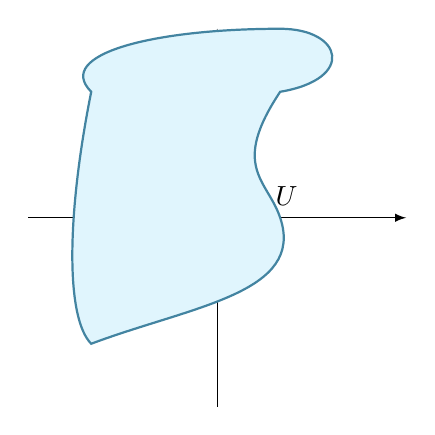
\begin{tikzpicture}[scale=0.8,>=latex]
  \draw[->] (-3,0)--(3,0); \draw[->] (0,-3)--(0,3);
  \filldraw[fill=cyan!12, draw=cyan!60!black, thick]
    (1,2) .. controls (2.2,2.2) and (2,3) .. (1,3)
    .. controls (-1,3) and (-2.6,2.6) .. (-2,2)
    .. controls (-2.4,0) and (-2.4,-1.6) .. (-2,-2)
    .. controls (-0.4,-1.4) and (1.4,-1.2) .. (1,0)
    .. controls (0.8,0.6) and (0.2,0.8) .. (1,2) -- cycle;
  \node at (1.1,0.35) {$U$};
\end{tikzpicture}
\end{document}
